\documentclass{article}
\usepackage[a4paper, total={6in, 10in}]{geometry}
\usepackage{multicol}
\usepackage{graphicx}
\usepackage{float}

\begin{document}

\title{Assessed Exercise 1: Microarchitecture Optimisation in Splay Trees}
\author{Charlie Lidbury}
\maketitle

\begin{multicols}{2}

  \section{Intro}
  There is a known set of controls we have over the microarchitecture of the SimpleScalar CPU, and we have the source code of the program being run.

  \section{Studying Microarchitectural Effects}
  At the start of the specification, there are a few direct questions, this section answers those.

  \begin{figure}[H]
    \centering
    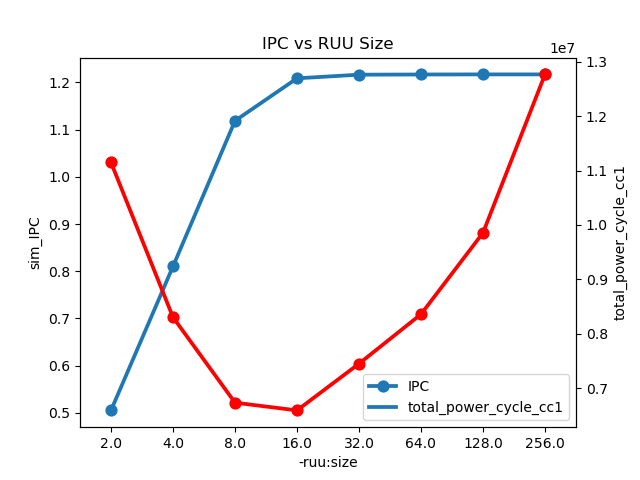
\includegraphics[width=\linewidth]{./assets/ipc_vs_ruu_size.png}
    \caption{IPC/Energy vs RUU Size}
    \label{fig:ipc_energy_vs_ruu}
  \end{figure}

  \subsection{Varying RUU}
  The more RUU you give the CPU, the more instructions per clock you get, likely because it can better utilize functional units, as shown in Figure \ref{fig:ipc_energy_vs_ruu}

  However, as shown by the red line, this does not translate to better energy efficiency forever. This is likely because the extra instructions per clock are not worth the extra energy cost of the larger RUU.

  \subsection{Varying both RUU and LSQ}
  If we vary both the RUU size and LSQ size at the same time, we can see that if either gets too small, the other becomes the bottleneck.

  \begin{figure}[H]
    \centering
    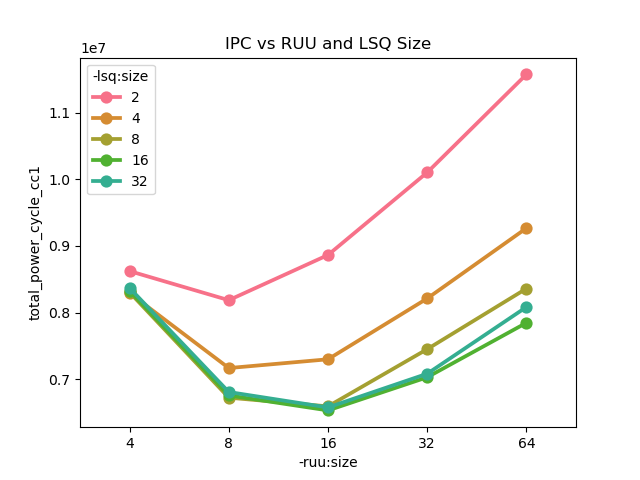
\includegraphics[width=\linewidth]{./assets/energy_vs_ruu_and_lsq_size.png}
    \caption{Energy vs RUU Size/LSQ Size}
    \label{fig:energy_vs_ruu_lsq}
  \end{figure}

  In Figure \ref{fig:energy_vs_ruu_lsq}, when the LSQ size is small, say 2, the optimal RUU size is 8. This is because the LSQ is the bottleneck, so the extra RUU space can't be utilized and it's just wasted energy. When there is more LSQ space, higher RUU numbers provide benefits.

  \subsection{Bottlenecks}
  Something is a bottleneck if increasing its size would speed up overall performance, so to investigate which components are bottlenecks, we can vary their size and see if it affects performance.

  We can alter the size/quantity of most components, but I'll assume for this question only the RUU and LSQ are under investigation.

  The default parameters are RUU=16 and LSQ=8, so I'll start there and increase. SimpleScalar doesn't seem to record simulated time, so I will assume that microarchitectural changes don't affect clock speed, and therefore the number of cycles is a good proxy for time.

  \begin{figure}[H]
    \centering
    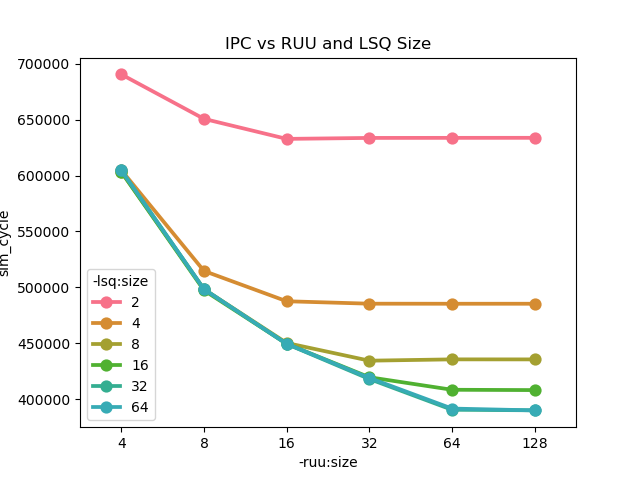
\includegraphics[width=\linewidth]{./assets/ruu_and_lsq_vs_sim_time.png}
    \caption{RUU and LSQ Increases vs performance}
    \label{fig:ruu_or_lsq_bottleneck}
  \end{figure}

  As shown in Figure \ref{fig:ruu_or_lsq_bottleneck}, which one is the bottleneck depends on the size of the other. If the RUU is small, the LSQ is the bottleneck, and vice versa.

  At the default parameters (RUU=16, LSQ=8) the LSQ seems to be the bottleneck because increasing the RUU past its default value of 16 doesn't increase performance. This is likely because the program has a lot of loads and stores, creating lots of entries in the LSQ.

  \subsection{Race-to-Finish Doesn't Always Win}
  As shown in Figure \ref{fig:energy_vs_ruu_lsq}, the RUU/LSQ configuration with the lowest energy usage in RUU=16, LSQ=16, Figure \ref{fig:ruu_or_lsq_bottleneck} shows it is \textit{at least} RUU=128, LSQ=64. Although there are diminishing returns, it looks like increasing the RUU and LSQ size always results in faster runtime.

  \section{Program Analysis}
  In this section, I will discuss the various microarchitecture parameters we can adjust, and how they will likely affect the execution of the given splay tree program.

  Splaytest inserts many elements into a splay tree, then reads many elements, as a random walk. Because it's a random walk, elements that have previously been accessed are very likely to be accessed again. The design of splay trees means many of these operations will be very fast, as the accessed key will have recently been \textit{splayed} over to the root.

  \subsection{Cache}
  \label{analysis:cache}
  The simulator allows us to adjust everything about the L1 and L2 cache (sets, block size, associativity, replacement strategy), as well as how many levels are unified between instructions and data.

  Looking at the splay tree code, it looks like each node is a struct with 4 8-byte fields, which probably means a cache block size of 32 bytes is optimal.

  \textbf{Spatial Locality} When the tree is splayed around a key, it does so by editing which nodes are pointing at which nodes; so it doesn't use an array representation/physically relocate the nodes in memory. As a result, although the splaying allows a recently accessed element to be accessed with fewer dereferences, it doesn't make the locality of the nodes any better. This means the over-fetching you get with big cache line sizes won't be useful here. I suspect this will make small cache lines more effective, as they require less energy and we wouldn't benefit from the over-fetching from a larger cache line.

  \textbf{Temporal Locality} The random walk means recently accessed elements are likely to be accessed again, which correlates directly to temporal locality. This program will likely exhibit good temporal locality.

  Perhaps this will mean we won't need as big a cache, as we will get a large hit rate?

  \subsection{Branch Prediction}
  We have control over what type of branch predictor is used and its config, as well as the config of the BTB. This is an integer program with a high branching factor, which will probably make speculative execution and branch prediction less effective than they typically are.

  \subsection{Functional Units}
  We can control how many integer/floating point ALUs/multipliers we have.

  Hardware dedicated to floating point operations will likely go almost entirely unused and do nothing but waste energy. The rest of the units will be a case of putting in \textit{just} enough to maximize utilization.

  \subsection{Multiple Instructions/Clock}
  We can alter how many instructions are decoded/issued/committed per cycle, which will affect the IPC, as well as the pressure placed on the other units. For instance, issuing lots of instructions per cycle means we can better utilize our functional units.

  \section{Experimentation}
  This section is split into two parts.

  In the first section, I will program specific information to find a set of reasonable variables; for instance, because I know there are very few floating point units I can reduce the number of those to 1 without worrying too much about its implications on the other functional units.

  In the second section, I will use pure parameter search to make sure I'm in a local minimum. By the end of this section, any parameter change should make the energy usage worse.

  \subsection{Informed Parameter Selection}

  \subsubsection{Cache}
  \subsubsection{L1 Block Size}
  \begin{figure}[H]
    \centering
    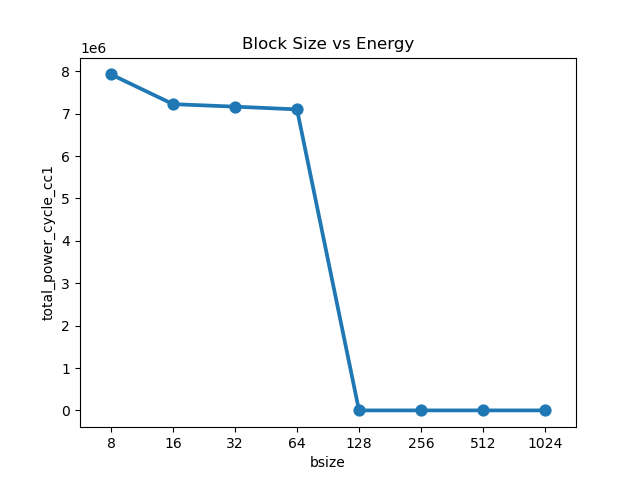
\includegraphics[width=\linewidth]{./assets/l1bsize_vs_energy.png}
    \caption{Energy vs Block Size}
    \label{fig:bsize_vs_energy}
  \end{figure}
  As discussed in section \ref{analysis:cache}, the nodes in the splay tree are 32 bytes, so if the cache block size is set to 32 bytes, it won't over or underfetch data when accessing a node. To test this, we vary the cache block size while keeping the total cache size constant. As shown in Figure \ref{fig:bsize_vs_energy}.


  This analysis shows when block size reaches 128B, the energy usage falls off a cliff, I assume this is a bug so I will take 32B as my block size.

  \subsubsection{L1 Cache Size}

  \begin{figure}[H]
    \centering
    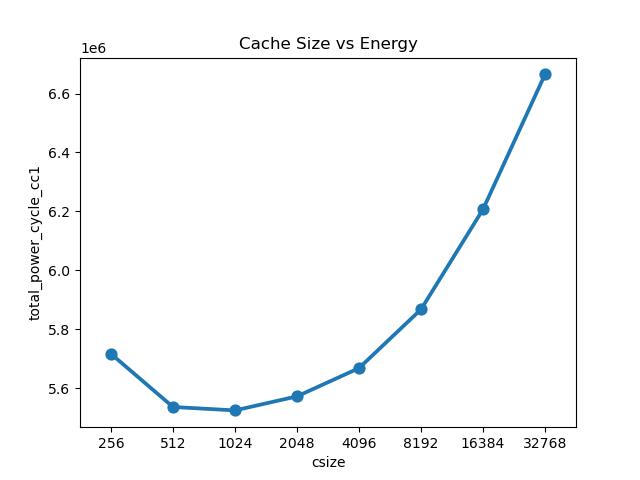
\includegraphics[width=\linewidth]{./assets/l1csize_vs_energy.png}
    \caption{Energy vs L1 Size}
    \label{fig:l1size_vs_energy2}
  \end{figure}

  With the block size minimized, we should be able to reduce the cache size until we start to see a performance hit. Figure \ref{fig:l1size_vs_energy2} shows we can reduce the cache size from 16k to 1k while still reducing energy. This is likely because the random walk means we get a good temporal locality, so we don't need a large cache.

  With this lower cache size, the optimal block size is still 32B. You might think that 64B would be counterproductive now that we have such a limited cache, but it only uses marginally more energy.

  \subsubsection{Functional Units}
  The only arithmetic-heavy thing in our program is the random number generation, so we should be able to reduce the number of functional units without affecting performance.

  To test this, I will change the amount of each functional unit individually to see if it makes a difference.

  \begin{figure}[H]
    \centering
    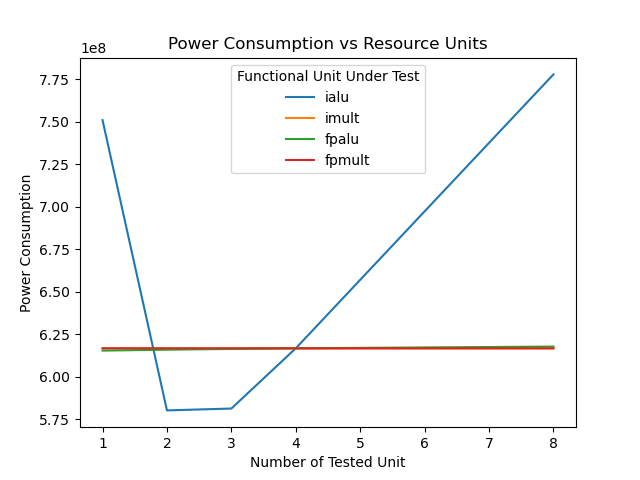
\includegraphics[width=\linewidth]{./assets/units_vs_energy.png}
    \caption{Functional Units vs Energy}
    \label{fig:units_vs_energy}
  \end{figure}

  Figure \ref{fig:units_vs_energy} shows the only functional unit that makes any difference is the integer ALU, which is best at 2. This makes sense as the other units are barely used, but the integer ALU is used for random number generation.

\end{multicols}

\end{document}
